\documentclass{article}

%% PAQUETES

% Paquetes generales
\usepackage[margin=2cm, paperwidth=210mm, paperheight=297mm]{geometry}
\usepackage[spanish]{babel}
\usepackage[utf8]{inputenc}
\usepackage{gensymb}

% Paquetes para estilos
\usepackage{textcomp}
\usepackage{setspace}
\usepackage{colortbl}
\usepackage{color}
\usepackage{color}
\usepackage{upquote}
\usepackage{xcolor}
\usepackage{listings}
\usepackage{caption}
\usepackage[T1]{fontenc}
\usepackage[scaled]{beramono}

% Paquetes extras
\usepackage{amssymb}
\usepackage{float}
\usepackage{graphicx}

%% Fin PAQUETES


% Definición de preferencias para la impresión de código fuente.
%% Colores
\definecolor{gray99}{gray}{.99}
\definecolor{gray95}{gray}{.95}
\definecolor{gray75}{gray}{.75}
\definecolor{gray50}{gray}{.50}
\definecolor{keywords_blue}{rgb}{0.13,0.13,1}
\definecolor{comments_green}{rgb}{0,0.5,0}
\definecolor{strings_red}{rgb}{0.9,0,0}

%% Caja de código
\DeclareCaptionFont{white}{\color{white}}
\DeclareCaptionFont{style_labelfont}{\color{black}\textbf}
\DeclareCaptionFont{style_textfont}{\it\color{black}}
\DeclareCaptionFormat{listing}{\colorbox{gray95}{\parbox{16.78cm}{#1#2#3}}}
\captionsetup[lstlisting]{format=listing,labelfont=style_labelfont,textfont=style_textfont}

\lstset{
	aboveskip = {1.5\baselineskip},
	backgroundcolor = \color{gray99},
	basicstyle = \ttfamily\footnotesize,
	breakatwhitespace = true,   
	breaklines = true,
	captionpos = t,
	columns = fixed,
	commentstyle = \color{comments_green},
	escapeinside = {\%*}{*)}, 
	extendedchars = true,
	frame = lines,
	keywordstyle = \color{keywords_blue}\bfseries,
	language = Octave,                       
	numbers = left,
	numbersep = 5pt,
	numberstyle = \tiny\ttfamily\color{gray50},
	prebreak = \raisebox{0ex}[0ex][0ex]{\ensuremath{\hookleftarrow}},
	rulecolor = \color{gray75},
	showspaces = false,
	showstringspaces = false, 
	showtabs = false,
	stepnumber = 1,
	stringstyle = \color{strings_red},                                    
	tabsize = 2,
	title = \null, % Default value: title=\lstname
	upquote = true,                  
}

%% FIGURAS
\captionsetup[figure]{labelfont=bf,textfont=it}

% COMANDOS

%% Titulo de las cajas de código
\renewcommand{\lstlistingname}{Código}
%% Titulo de las figuras
\renewcommand{\figurename}{Figura}
%% Referencia a los códigos
\newcommand{\refcode}[1]{\textit{Código \ref{#1}}}
%% Referencia a las imagenes
\newcommand{\refimage}[1]{\textit{Imagen \ref{#1}}}



\begin{document}

% Inserción del título, autores y fecha.
\title{\huge 61.09 Probabilidad y Estadística \\ 
	  \Huge Trabajo Práctico de Simulación \\
	  \bigskip \Large 13 de mayo de 2012 \\
	  \bigskip \large \textbf{Grupo 1} \\
	  \large \textit{Loiza, Samanta (91935)\\Aguilera, Juan Martín (92483)\\Rossi, Federico Martín (92086)}}
\date{}
\maketitle


% INTRODUCCIÓN

\section{Introducción}

	Con el fin de fortalecer las nociones fundamentales de la probabilidad es que este trabajo busca aplicar las bases de los conceptos ya estudiados en el curso de manera tal de adoptar una mejor comprensión de la inferencia estadística en hechos cotidianos. En este caso, nuestro trabajo será explorar las propiedades estádisticas de cierto tipo de secuencias, las cuales serán detalladas más adelante.
	\par 
	En cada análisis realizado se mostrará su resolución analítica, como así también algoritmos que simulen dichas situaciones, a fin de poder mostrar una aproximación a la constatación empírica de los resultados. Estos últimos se han hecho en el lenguaje de programación \textit{GNU Octave}\footnote{``\textit{GNU Octave} es un lenguaje interpretado de alto nivel, pensado principalmente para cálculos numéricos. Para más información dirijase a \textit{http://www.gnu.org/software/octave} ''}.
	\par 
	Todos los archivos y códigos fuente aquí mencionados, así como también el presente informe, pueden ser descargados de la sección \textit{Downloads} del repositorio del grupo (\textit{http://code.google.com/p/simulacion-proba2012}).



% ACTIVIDADES PREVIAS
\section{Actividades previas}

Tal como lo sugiere el título de este apartado, se mostrarán a continuación una serie de actividades previas necesarias para dominar las técnicas básicas de simulación de números aleatorios.


% ACTIVIDADES PREVIAS - Una primera simulación
\subsection{Una primera simulación}

A continuación, en el \refcode{code:punto1.1}, se muestra una rutina que, a partir de un generador de números pseudo-aleatorios, permite simular los valores de un dado. Como se puede ver, se ha utilizado la función nativa \textbf{\textit{rand}}, la cual devuelve una matriz (que es utilizada como vector) con valores aleatrios entre 0 y 1. Para ajustarla a nuestras necesidades, o sea, obtener valores aleatorios entre 1 y 6 hemos multiplicado dicho vector por 6. De esta manera pasa a contener valores aleatorios entre 0 y 6. Luego, mediante otra funcion nativa llamada \textbf{\textit{ceil}}, se redondea a los valores enteros próximos superiores de cada uno (ceiling), obteniendo como resultado un vector con valores enteros entre 1 y 6. 

% Código
\lstinputlisting[label=code:punto1.1,caption=randomDado.m]{source/randomDado.m}

\medskip
\par
Por lo explicado anteriormente, es evidente que como a cada valor se lo trató de la misma manera, se puede decir que no alteramos los resultados del \textbf{\textit{rand}}, y por lo tanto la probabilidad de cada número sigue siendo la misma.
	\par
	Un detalle no menor a tener en cuenta es la gran importancia del criterio con el que se redondean los números ya que para consevar la equiprobabilidad de los valores hay que utilizar el mismo criterio para todos ellos.
	\par
	Habiendo conseguido valores aleatorios entre 1 y 6 mediante el procedimiento antes mencionado, ahora deseamos obtener valores aleatorios entre dos números enteros genéricos, o sea, a partir de un intervalo cualquiera. El problema radica ahora en que si ninguno de los extremos es el 0, los valores no caen dentro del intervalo esperado y, por ende, habría que desplazar el intervalo. Por lo tanto, una forma de conseguir números enteros aleatorios en un intervalo genérico es, primero, calcular los números aleatorios entre 0 y la longitud del intervalo requerido más uno (porque se redondea para arriba). Luego, hay que sumarle el extremo inferior menos uno, obteniendo así números enteros aleatorios dentro del intervalo esperado. Este método es el utilizado en el algoritmo del \refcode{code:punto1.2}.

% Código
\lstinputlisting[label=code:punto1.2,caption=randomGenerico.m]{source/randomGenerico.m}
\bigskip


% ACTIVIDADES PREVIAS - Puesta a prueba
\subsection{Puesta a prueba}

Pondremos a prueba ahora lo visto en el apartado anterior estimando las probabilidades de cada uno de los 6 valores posibles utilizando los resultados obtenidos en 1000 ejecuciones de la rutina. Para comprobar que el algoritmo planteado funciona, se creo otra función que cuenta las apariciones de un número en un vector de números \textit{probNum(n,vector)}\footnote{``\textit{Véase el Apéndice, sección 4.x}''}. La salida por pantalla de la ejecución es: \\

{\ttfamily\footnotesize
\indent tiradasDado = randomDado(1000);\\
\indent octave:2> prob1 = probNum(1,tiradasDado)\\
\indent prob1 =  0.16200 \\
\indent octave:3> prob2 = probNum(2,tiradasDado)\\
\indent prob2 =  0.17800\\
\indent octave:4> prob3 = probNum(3,tiradasDado)\\
\indent prob3 =  0.17700\\
\indent octave:5> prob4 = probNum(4,tiradasDado)\\
\indent prob4 =  0.17000\\
\indent octave:6> prob5 = probNum(5,tiradasDado)\\
\indent prob5 =  0.15800\\
\indent octave:7> prob6 = probNum(6,tiradasDado)\\
\indent prob6 =  0.15500\\
\indent octave:8> prob1 + prob2 + prob3 + prob4 + prob5 + prob6\\
\indent ans =  1\\}

Se puede ver que las probabilidades de que salga cada número, no son exactamente las esperadas, pero se acercan a este valor. Téngase en cuenta que cuanto mayor es el número de ejecuciones, las probabilidades se van acercando más al valor calculado teóricamente. \\
En el siguiente diagrama se puede ver como la cantidad de apariciones de los valores del dado  para 1000 tiradas se distribuye entre todos los valores. 

\begin{figure}[h]
	\centering
	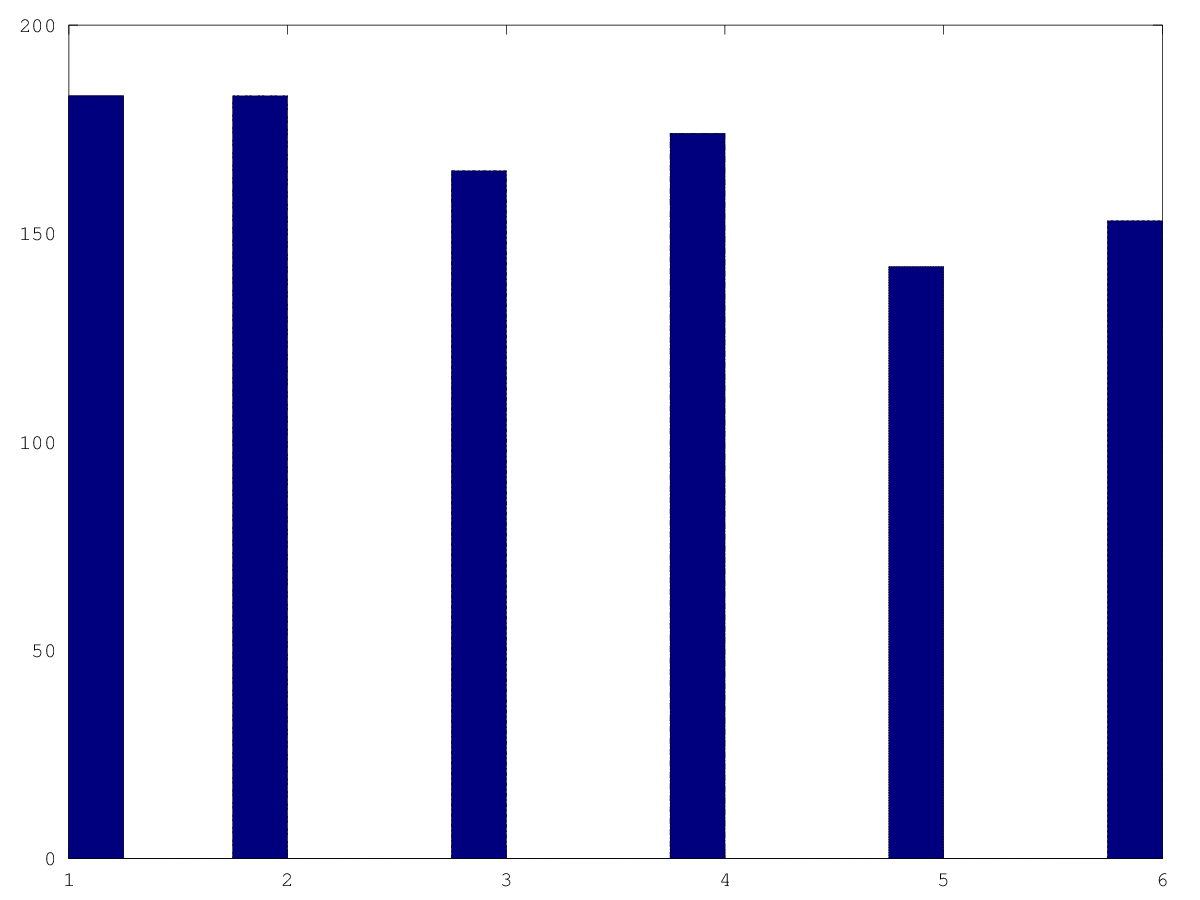
\includegraphics[width=0.60\textwidth]{images/probabilidadesDados.png}
	\caption{Cantidad de veces que sale cada valor de un dado en 1000 lanzamientos de este.}
\end{figure}
\bigskip



% ACTIVIDADES PREVIAS - Predicados
\subsection{Predicados}

A veces se necesita estimar la probabilidad de un evento definido a partir de variables aleatorias. Por ejemplo, supongamos que deseamos estimar la probabilidad de que al tirar dos dados, uno tenga el doble de valor que el otro. Para esto proponemos la siguiente solución analítica:\\

% Desarrollo de cuentas
\indent $\Omega = \{1,2,3,4,5,6\}$ \\

\indent M: ``Valor del Dado 1''\\
\indent N: ``Valor del Dado 2''\\

\indent $\mathbb{P}(M=1, N=2) = ({1 \over 6})^2$ \medskip\\
\indent $\mathbb{P}(M=2, N=4) = ({1 \over 6})^2$ \medskip\\
\indent $\mathbb{P}(M=3, N=6) = ({1 \over 6})^2$ \medskip\\

\indent $\Rightarrow \mathbb{P}(N=2M) = 3\cdot({1 \over 36}) = {3 \over 36} \thickapprox 0.08\hat{3}\\$
 % FIN % Desarrollo de cuentas

\noindent Como se puede observar en el desarrollo anterior, solo son tres los casos en los que se cumple que N = 2M. El lector se habrá dado cuenta de que esta probabilidad no considera todos los casos posibles ya que falta considerar los casos en que M = 2N. De todas maneras, el cálculo de la probabilidad de esta última expresión no es dificil, ya que dicha probabilidad posee el mismo valor que $\mathbb{P}(N=2M)$. Por si el lector no se encuentra convencido de esto último, veamos:\\

% Desarrollo de cuentas
\indent $\mathbb{P}(M=2, N=1) = ({1 \over 6})^2$ \medskip\\
\indent $\mathbb{P}(M=4, N=2) = ({1 \over 6})^2$ \medskip\\
\indent $\mathbb{P}(M=6, N=3) = ({1 \over 6})^2$ \medskip\\

\indent $\Rightarrow \mathbb{P}(M=2N) = 3\cdot({1 \over 36}) = {3 \over 36} \thickapprox 0.08\hat{3}\\$
 % FIN % Desarrollo de cuentas

\medskip
\noindent Por lo tanto podemos decir que $\mathbb{P}(N=2M) = \mathbb{P}(M=2N) \thickapprox 0.08\hat{3}$.
	\par
	Ahora, el propósito nuestro es obtener $\mathbb{P}[(N=2M) \cup (M=2N)]$, pero si observamos fijamente, podemos ver que ambos eventos de la unión son disjuntos entre sí, por lo que resulta:\\

\indent $\mathbb{P}[(N=2M) \cup (M=2N)] = \mathbb{P}(N=2M) + \mathbb{P}(M=2N) = {3 \over 36} + {3 \over 36} = 2({3 \over 36}) = {6 \over 36} = {1 \over 6} \thickapprox 0.1\hat{6}  $ \medskip\\

	\par
	Para constatar el resultado obtenido proponemos la rutina mostrada en el \refcode{code:punto3} la cual simula la situación planteada. En este, como en la mayor parte de los otros casos, se utiliza la lógica de casos favorables sobre casos posibles para poder determinar el valor de probabilidad buscado. Es decir, se generan valores de dados al azar (simulando ser tiradas), se cuentan cuantos cumplen con lo propuesto y a este valor se lo divide por la cantidad total de veces que se generaron valores. Al correr esta función para \textit{n=1000000}, siendo \textit{n} la \textit{cantidad de tiradas a simular}, se obtuvo que $\mathbb{P}[(N=2M) \cup (M=2N)] = 0.16663$, lo cual es bastante aproximado al valor obtenido analíticamente.

% Código
\lstinputlisting[label=code:punto3,caption=probDobleDelOtro.m]{source/probDobleDelOtro.m}
\bigskip


% ACTIVIDADES PREVIAS - Enigma final
\subsection{Enigma final}

Con lo hecho y aprendido hasta ahora podemos plantearnos la misma pregunta que se hizo a sí mismo el Caballero de Méré en el siglo XVII: 

\begin{quotation}
\em``¿Cómo puede ser que cuando apuesto a que voy a obtener al menos un doble As en 24 tiradas de dos dados suelo perder, siendo que suelo ganar cuando apuesto a que voy a obtener al menos un As en 4 tiradas?''
\end{quotation}

\noindent Para analizar esta especie de acertijo, primeramente tengamos en cuenta que, definiendo \textit{S} y \textit{NS} como\\

\indent \textit{S: ``Sale As en una tirada del dado''}\\
\indent \textit{NS: ``No sale As en una tirada del dado''}\\

\noindent sabemos que, $\mathbb{P}(S) = {1 \over 6}$ y $\mathbb{P}(NS) = {5 \over 6}$. 
Para calcular la \textit{probabilidad de obtener al menos un doble As en 24 tiradas de dos dados} podemos plantear analíticamente lo que sigue:\\

% Desarrollo de cuentas
\indent \textit{X: ``Cantidad de Ases en una tirada de los dos dados''}\\
\indent $\Omega(X) = \{0,1,2\}$ \\

\indent $\mathbb{P}(X=0) = ({1 \over 36})5 = {5 \over 36}$ \medskip\\
\indent $\mathbb{P}(X=1) = ({1 \over 6}{5 \over 6})6 = {5 \over 6}$ \medskip\\
\indent $\mathbb{P}(X=2) = {1 \over 6}{1 \over 6} = {1 \over 36}$ \medskip\\

\noindent De esto podemos deducir fácilmente que,\\

\indent $\mathbb{P}(X \neq 2) = {35 \over 36}$ \medskip\\
\indent $\mathbb{P}(\Omega) = {5 \over 36} + {5 \over 6} + {1 \over 36} = 1$ \medskip\\

\noindent Entonces, definiendo \textit{A} como sigue, resulta:\\

\indent \textit{A: ``Obtener al menos un doble As en 24 tiradas de dos dados.''}\\
\indent \textit{$\bar{A}$: ``No obtener ningún doble As en 24 tiradas de dos dados.''}\\

$\mathbb{P}(A) = 1 - \mathbb{P}(\bar{A}) = 1 - [\mathbb{P}(X \neq 2)]^{24} = 1- ({35 \over 36})^{24} \thickapprox 0.4914$ \medskip\\
 
En este resultado se puede observar que las probabilidades de obtener al menos un doble As en 24 tiradas de dos dados es aproximadamente del 50\%. Para verificar la validez de este resultado, en el \refcode{code:punto4.1} se muestra un algoritmo que simula dicha situación.  Con este hemos obtenido que, para un número de repeticiones \mbox{\textit{n = 1000000}}, $\mathbb{P}(A) = 0.49189$, el cual es un valor muy cercano al calculado analíticamente.

% Código
\lstinputlisting[label=code:punto4.1,caption=probDobleAsEn24Tiradas.m]{source/probDobleAsEn24Tiradas.m} 
\bigskip\bigskip

	Ahora bien, para calcular la \textit{probabilidad de obtener al menos un As en 4 tiradas} podemos plantear la siguiente solución analítica:\\

% Desarrollo de cuentas
\indent \textit{B: ``Obtener al menos un As en 4 tiradas''}\\
\indent \textit{$\bar{B}$: ``No Obtener ningún As en 4 tiradas''}\\

$\mathbb{P}(B) = 1 - \mathbb{P}(\bar{B}) = 1- ({5 \over 6})^4 = \thickapprox 0.51775$\\\bigskip

\noindent Como se puede observar, la probabilidad de no obtener ningún As en una tirada es igual a la multiplicación de las probabilidades de no obtener As en la tirada de un dado. Esto se debe a que estos eventos son independientes entre sí, lo que nos posibilita hacer el cálculo de esa forma. Para constatar los cálculos empíricamente presentamos el \refcode{code:punto4.2} que simula dicha situación. Con este hemos obtenido que, para un número de repeticiones \mbox{\textit{n = 1000000}}, $\mathbb{P}(B) = 0.51759$, el cual es un valor bastante aproximado a lo obtenido analíticamente.

% Código
\lstinputlisting[label=code:punto4.2,caption=probAsEn4Tiradas.m]{source/probAsEn4Tiradas.m}
\bigskip

Teniendo los dos resultados de las probabilidades a la vista, no es claro ver el por qué de que el Caballero de Méré suela perder cuando apuesta a que va a obtener al menos un doble As en 24 tiradas de dos dados y que suela ganar cuando apuesta a que va a obtener al menos un As en 4 tirada, ya que las probabilidades de ambos casos  son parecidas. De todas formas, estos números son viables para una cantidad de repeticiones alta, por lo que para pocas experiencias, podría ser que pierda más veces de las que gane.
\bigskip




% ACTIVIDAD PRINCIPAL
\section{Actividad principal}

	Primeramente veamos la situación a analizar. Luego de haber escrito una pieza de software, se desea someterlo a una prueba que garantice su funcionamiento para todas las entradas posibles (finitas). Dado que cada ejecución puede ser afectada por los resultados de las anteriores, se descartan los métodos triviales que consistan en probarlas siguiendo un patrón preestablecido.
	Atendiendo a lo anterior, se propone elegir al azar una entrada con la cual realizar la ejecución y repetir el procedimiento hasta que todas hayan sido elegidas al menos una vez. Si por ejemplo, existen 3 entradas posibles, representadas por los dígitos 1, 2 y 3, las secuencias que se muestran a continuación serían válidas:

\begin{itemize}
\itemsep=2pt \topsep=0pt \partopsep=0pt \parskip=0pt \parsep=0pt
	\item 3 2 2 2 3 3 2 2 3 2 2 2 3 2 3 1
	\item 1 1 2 3
	\item 1 3 2
	\item 2 1 2 2 2 2 3
\end{itemize}

	Es importante remarcar que en cada paso se elige cualquiera sin importar si ya había sido elegida e independientemente de los valores obtenidos anteriormente. Como se puede apreciar, las longitudes de estas secuencias (y por lo tanto, el tiempo y la memoria que consumen) son aleatorias.
	\par 
	Habiendonos situado en lo recién expuesto, pasaremos a explorar y analizar las propiedades estadísticas de las secuencias generadas.



% ACTIVIDAD PRINCIPAL - Algoritmo generador de secuencias
\subsection{Algoritmo generador de secuencias}

En el \refcode{code:punto5} se puede observar el algoritmo que simula la situación antes mencionada. Este es capaz de simular muchas veces las secuencias de entradas descritas, siendo posible la especificación la cantidad de entradas posibles (\textit{M}) y la cantidad de secuencias a generar (\textit{N}).

% Código
\lstinputlisting[label=code:punto5,caption=generaSecuencias.m]{source/generaSecuencias.m}
\bigskip

% ACTIVIDAD PRINCIPAL - Análisis del algoritmo
\subsection{Análisis del algoritmo}

	Si se asume que \textit{L} es una variable aleatoria, entonces el método para calcular el valor de longitud esperado, o la longitud media, se extrae del cálculo de la esperanza para una variable aleatoria discreta. Esto es:\\
	 
$\mathbb{E}(\textit{L}) = \sum\limits_{i=1}^n l_{i} \mathbb{P}_{i}(l_{i}) $

\bigskip
\noindent con \textit{n} la cantidad de secuencias, y siendo \textit{$l_i$} la longitud de la secuencia \textit{i} y \textit{$\mathbb{P}(l_i)$} la probabilidad de \textit{$l_i$}. Ya que vimos que los números generados son equiprobables, entonces las longitudes de las secuencias tambien, y por lo tanto tienen probabilidad $1 \over n$, y se puede simplificar la fórmula a:\\

\indent $\mathbb{E}(\textit{L}) = {1 \over n} \sum\limits_{i=1}^n l_{i} $,

\bigskip
\noindent que es lo mismo, la suma de las longitudes dividido la cantidad de secuencias. 
	\par
	Este cálculo puede ser resuelto mediante el algoritmo mostrado en el \refcode{code:punto6}, el cual suma las longitudes de las secuencias contenidas en una lista (vector) pasado por parámetro a la función y luego divide el resultado de la suma por la cantidad total de secuencias albergadas en la lista, devolviéndonos la media buscada de la variable aleatoria \textit{L}.\medskip

% Código
\lstinputlisting[label=code:punto6,caption=esperanzaDeLaLongitud.m]{source/esperanzaDeLaLongitud.m}
\bigskip

\bigskip 
\noindent Para el caso de \textit{M = 10} y \textit{N = 1000}, el resultado obtenido fue el siguiente:\\

{\ttfamily\footnotesize
\indent octave:1> listaDeSecuencias = generaSecuencias(1000,10);\\
\indent octave:2> esperanzaDeLaLongitud(listaDeSecuencias)\\
\indent ans =  29.407}

\bigskip
En la \textit{Figura 2} se muestra un gráfico de las longitudes de las secuencias, en el que se puede apreciar que los valores de las longitudes son cercanos a la recta de la esperanza (marcada en rojo). Por lo tanto, podemos decir que el resultado del grafico concuerda con lo calculado. \\

\begin{figure}[h]
	\centering
	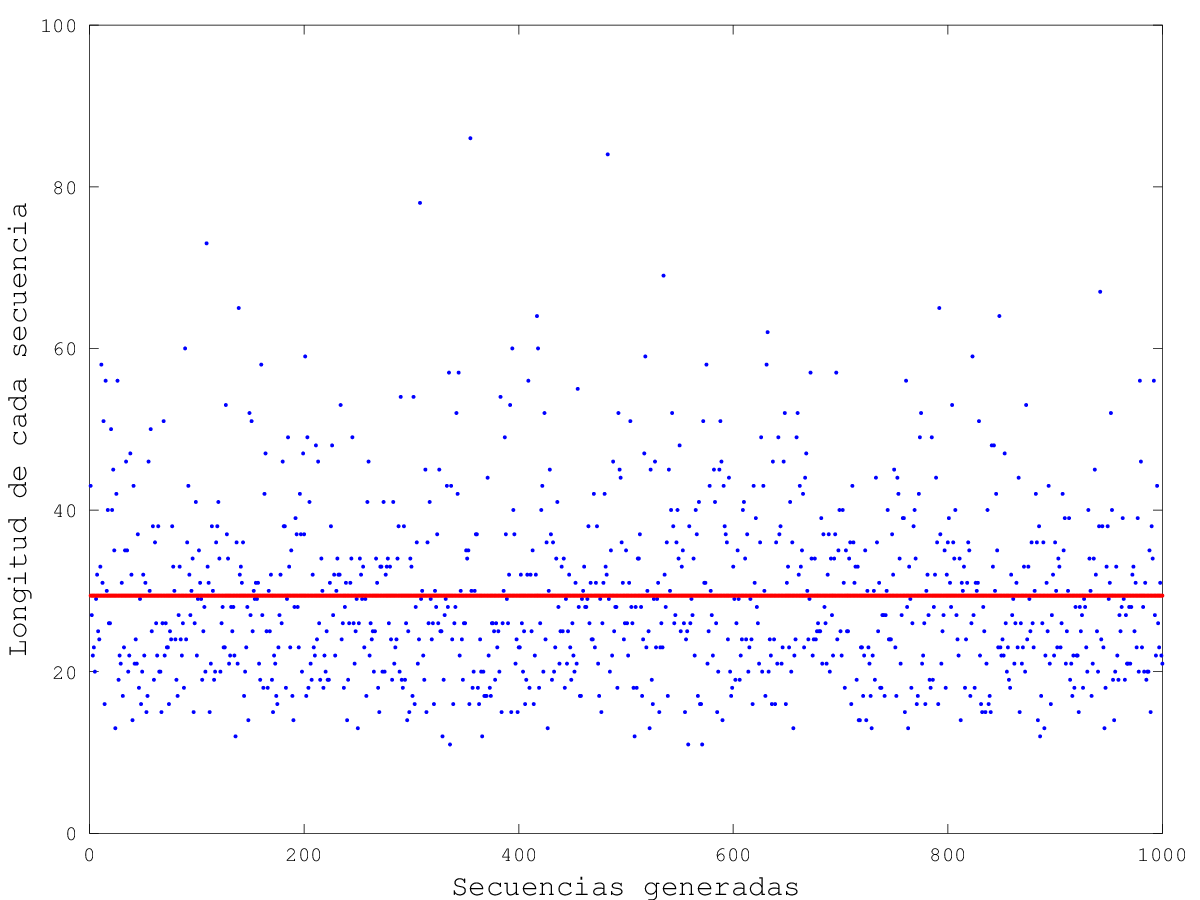
\includegraphics[width=0.80\textwidth]{images/longitudes.png}
	\caption{Longitudes de las secuencias.}
\end{figure}
\bigskip



% ACTIVIDAD PRINCIPAL - Probabilidad de los posibles valores de L
\subsection{Probabilidad de los posibles valores de \textit{L}}

Deseamos ahora estimar las probabilidades de los distintos valores posibles de \textit{L} a partir de los 1000 valores obtenidos en los apartados anteriores. Para esto se utilizó la rutina mostrada en el \refcode{code:punto7}, la cual, pasándole una lista de secuencias, calcula la probabilidad de cada una de las distintas longitudes de las secuencias contenidas en dicha lista.
	\par
	Como puede observarse, este algoritmo utiliza una función llamada \textit{probDeLaLongitud} para calcular las probabilidades individuales de cada longitud. Para más detalles sobre esta, véase el \textit{Apéndice}, \textit{sección 4.1.5}. Luego de procesar cada longitud se devuelve una matriz de dos columnas, siendo la primera la representativa de las longitudes y la segunda la representativa de las probabilidades de cada longitud.


% Código
\lstinputlisting[label=code:punto7,caption=probDeTodasLasLongitudes.m]{source/probDeTodasLasLongitudes.m}
\bigskip


\noindent Para una estimación hecha se han obtenido los siguientes valores de longitudes y probabilidades respectivas:\\

{\ttfamily\footnotesize
\indent octave:15> listaDeSecuencias = generaSecuencias(1000,10);\\
\indent octave:16> probDeTodasLasLongitudes(listaDeSecuencias)\\
\indent ans =\\

\indent    3.9000e+01   2.2000e-02\\
\indent    3.5000e+01   2.6000e-02\\
\indent    1.5000e+01   1.5000e-02\\
\indent    5.7000e+01   5.0000e-03\\
\indent    3.4000e+01   1.9000e-02\\
\indent    2.0000e+01   3.9000e-02\\
\indent    2.4000e+01   3.4000e-02\\
\indent    1.9000e+01   3.6000e-02\\
\indent    3.2000e+01   2.7000e-02\\
\indent    1.3000e+01   9.0000e-03\\
\indent    2.9000e+01   3.0000e-02\\
\indent    4.6000e+01   7.0000e-03\\
\indent    1.8000e+01   3.7000e-02\\
\indent    2.7000e+01   5.2000e-02\\
\indent    2.6000e+01   4.7000e-02\\
\indent    3.3000e+01   1.5000e-02\\
\indent    5.1000e+01   3.0000e-03\\
\indent    2.5000e+01   4.6000e-02\\
\indent    1.6000e+01   2.4000e-02\\
\indent    5.4000e+01   5.0000e-03\\
\indent    3.0000e+01   3.9000e-02\\
\indent    2.2000e+01   5.2000e-02\\
\indent    3.8000e+01   1.8000e-02\\
\indent    2.3000e+01   5.3000e-02\\
\indent    3.1000e+01   3.3000e-02\\
\indent    4.0000e+01   1.5000e-02\\
\indent    6.9000e+01   3.0000e-03\\
\indent    1.7000e+01   3.4000e-02\\
\indent    4.8000e+01   1.4000e-02\\
\indent    2.8000e+01   2.8000e-02\\
\indent    3.6000e+01   2.6000e-02\\
\indent    7.2000e+01   2.0000e-03\\
\indent    2.1000e+01   3.1000e-02\\
\indent    5.5000e+01   5.0000e-03\\
\indent    1.1000e+01   4.0000e-03\\
\indent    5.8000e+01   4.0000e-03\\
\indent    1.2000e+01   8.0000e-03\\
\indent    4.3000e+01   1.1000e-02\\
\indent    3.7000e+01   1.7000e-02\\
\indent    7.9000e+01   1.0000e-03\\
\indent    4.1000e+01   8.0000e-03\\
\indent    6.2000e+01   2.0000e-03\\
\indent    4.2000e+01   1.2000e-02\\
\indent    4.5000e+01   9.0000e-03\\
\indent    4.7000e+01   8.0000e-03\\
\indent    5.3000e+01   6.0000e-03\\
\indent    4.4000e+01   1.1000e-02\\
\indent    1.4000e+01   1.4000e-02\\
\indent    5.0000e+01   8.0000e-03\\
\indent    6.0000e+01   4.0000e-03\\
\indent    5.6000e+01   5.0000e-03\\
\indent    5.2000e+01   3.0000e-03\\
\indent    6.4000e+01   2.0000e-03\\
\indent    4.9000e+01   1.0000e-03\\
\indent    6.5000e+01   3.0000e-03\\
\indent    6.3000e+01   1.0000e-03\\
\indent    7.0000e+01   2.0000e-03\\
\indent    6.8000e+01   1.0000e-03\\
\indent    7.5000e+01   1.0000e-03\\
\indent    6.6000e+01   1.0000e-03\\
\indent    5.9000e+01   1.0000e-03\\
\indent    7.1000e+01   1.0000e-03\\
}



% ACTIVIDAD PRINCIPAL - Probabilidad de los posibles valores de L
\subsection{Una última cuestión}

Por último, supongamos que por razones de previsibilidad no se pueden generar secuencias más largas que una determinada longitud. Entonces, ¿será razonable proponer como límite el doble de \textit{M}?
	\par
	Dado al gráfico obtenido de las longitudes de las secuencias y de la esperanza calculada, se puede demostrar claramente que los resultados dan muy por encima del doble de la cantidad de entradas posibles. Aplicado al caso \textit{M=10}, los valores dan en su mayoría por encima de 20 (el doble de \textit{M}). Además, la esperanza da un valor aproximado de 29, también por encima de 2M. Esto se ha probado para otros posibles valores de \textit{M}, cuyos resultados coinciden con la experiencia anterior. El valor de la esperanza (promedio ponderado) de la longitud da mayor al doble de número de entradas, por lo que \textit{no es razonable proponer a L = 2M cómo el máximo de longitud de las secuencias}. Esto es comprobado gracias a la experiencia realizada en el trabajo.




% APENDICE
\section{Apéndice}


% APENDICE - Algoritmos relevantes
\subsection{Algoritmos relevantes}

En las siguientes secciones se detalla el funcionamiento de las funciones genéricas utilizadas para realizar los algoritmos de simulación.


\subsubsection{rand()}

Esta función de redondeo utiliza el algoritmo \textit{Mersenne Twister}\footnote{``\textit{http://www.math.sci.hiroshima-u.ac.jp/~m-mat/MT/emt.html}''}.


\subsubsection{ceil(n)}

Esta función de \textit{GNU Octave} devuelve el primer número entero no menor al número \textit{n}.


\subsubsection{probNum(n,vector)}

Este algoritmo (\refcode{code:punto8}) cuenta la cantidad de apariciones de un número 'n' en el 'vector', y luego lo divide por el largo del vector. Si suponemos que esos números en el vector son elegidos aleatoriamente, entonces lo que devuelve la función es la probabilidad de aparición de n.

% Código
\lstinputlisting[label=code:punto8,caption=probNum.m]{source/probNum.m}


\subsubsection{histogramaDeLaEsperanzaDeLaLongitud(listaDeSecuencias)}

Esta función (\refcode{code:punto9}) grafica los valores de la longitud de la secuencias que hay en la 'listaDeSecuencias'. Además grafica la esperanza de la longitud.

% Código
\lstinputlisting[label=code:punto9,caption=histogramaEsperanzaDeLaLongitud.m]{source/histogramaEsperanzaDeLaLongitud.m}


\subsubsection{probDeLaLongitud(longitud,listaDeSecuencias)}

Esta función (\refcode{code:punto10}) calcula la probabilidad de la longitud de una secuencia ubicada dentro de una lista de secuencias.

% Código
\lstinputlisting[label=code:punto10,caption=probDeLaLongitud.m]{source/probDeLaLongitud.m}
\bigskip


\end{document}
